\chapter{Technical contributions}
\label{chapter:technical}
% / Automatic Diversity for Wasm/ 


% The need for technical contributions...
We aim to create Artificial Software Diversity for \wasm, by providing tools to make the process easier and feasible for developers and researchers. As far as we know, there is no software that provides Artificial Software Diversification for WebAssembly. Therefore, we need to enunciate the engineering foundation to implement the strategies in \autoref{sota:sota}. Our implementations are part of the contributions of this thesis. Concretely, we provide two software artifacts that complement this work. Our approaches generate \wasm program variants statically at compile time to provide randomization. Besides, it also provides the tooling to generate MVE binaries for WebAssembly.


In this chapter we describe our technical contributions. In \autoref{tech:generic} we enunciate how the current state-of-the-art lead us to contribute with Software Diversification through LLVM. We follow by describing our two contributions and their main technical insights in \autoref{section:crow} and \autoref{section:mewe}. Besides, we describe a new transformation strategy as part of our contributions. 


% What does it solve ?
% The aim of massive-scale software diversity is to make it 

% . However, 

% In this chapter, we describe our threat model, return- and jump-oriented program- ming (see Section 4.2), new classes of code-reuse attacks. Code-reuse attacks are an attack class that is growing in popularity in response to other host-based defenses.
% Then we describe several compiler-based transformations (Section 4.3) and their im- plementation (Section 4.4) in the LLVM 2.9 compiler toolchain. We also provide some metrics (Section 4.5) for evaluating the effectiveness of these techniques for preventing wide-scale deployment of code-reuse attacks

%\todo{Make a real introduction, the paragraphs below is too fast}






\section{Global approach}
\label{tech:generic}


The work of Hilbig et al. \cite{Hilbig2021AnES} in 2021 influences our design decisions. According to their work, 70\% of the \wasm binaries in the wild are created with LLVM-based compilers. Therefore, we provide artificial software diversity for \wasm through LLVM. 
Other solutions would have been to diversify at the source-code level or the \wasm binary level. However, these facts would limit the applicability of our work.
Our approach is more general as diversification also will work for other LLVM backends.

LLVM is a compound of three main components \cite{llvmofficialweb}. First, the frontend (compilers such as clang and rustc) converts the program source code to LLVM intermediate representation (LLVM IR). Second, optimization and transformation processes improve the LLVM IR. Third and final, the backend component is in charge of generating the target machine code. In \autoref{diagrams:generic} we show how we use the LLVM pipeline in our contributions, which are highlighted as dashed squares.

\begin{figure*}[h]
    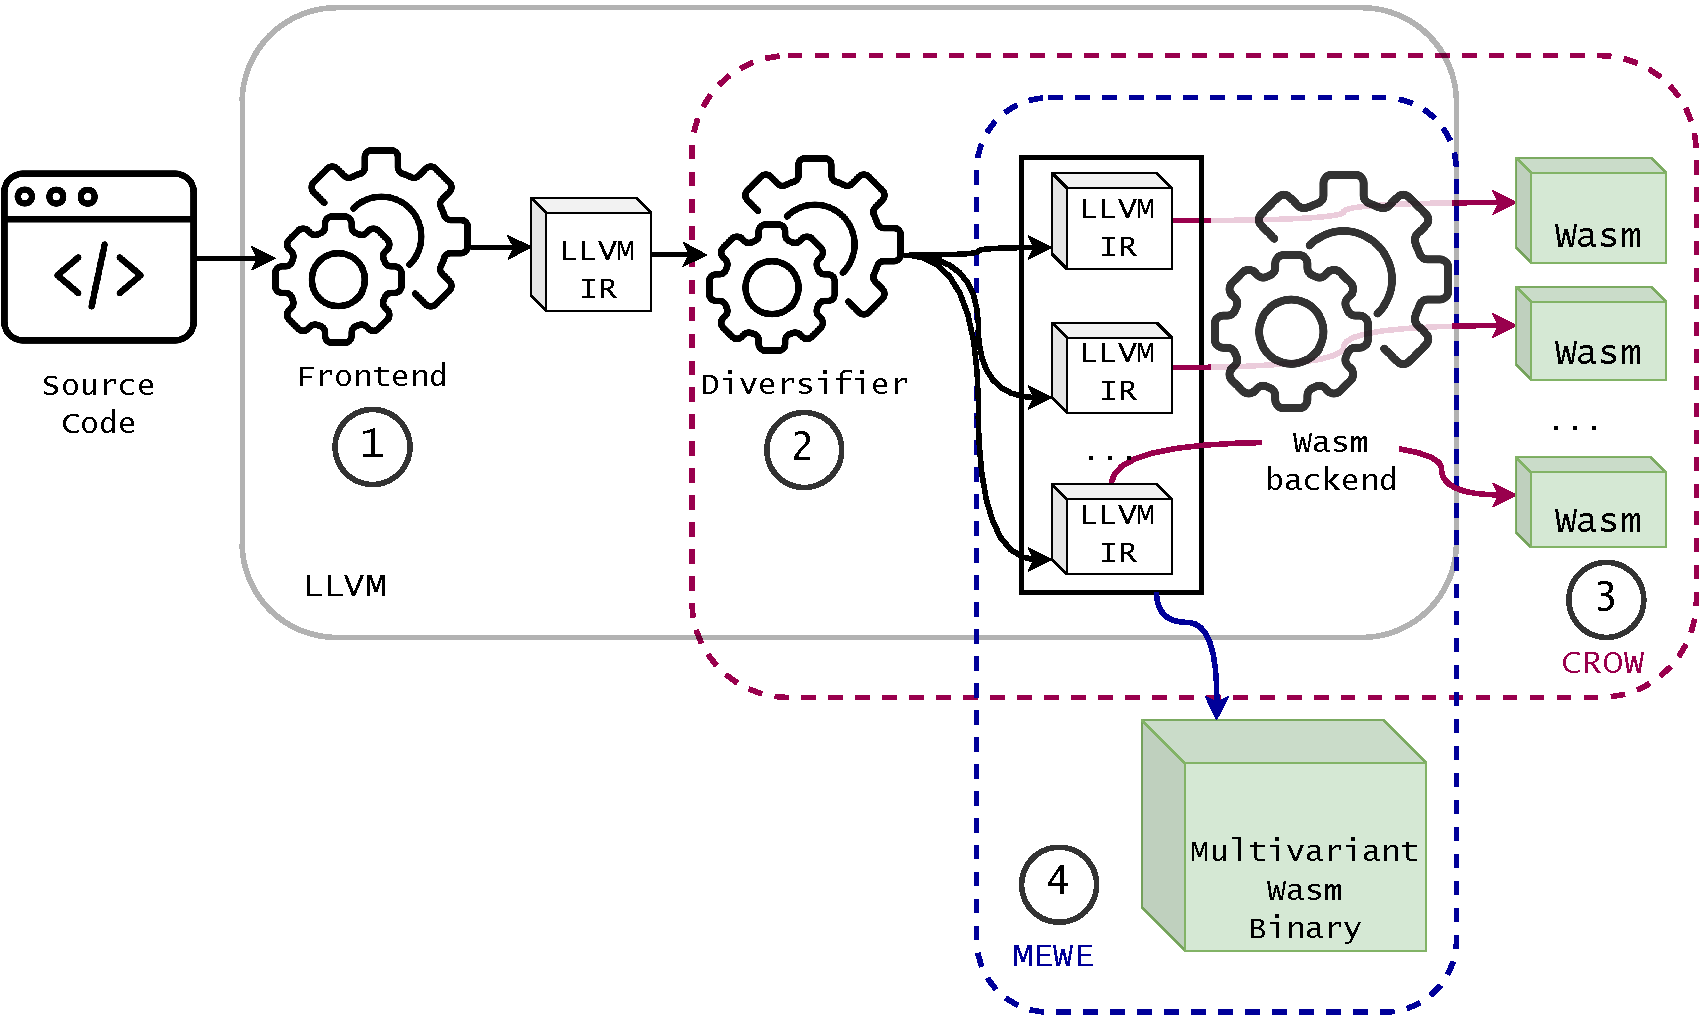
\includegraphics[width=\linewidth]{diagrams/architecture.pdf}
    \caption{Generic workflow to create \wasm program variants.}
    \label{diagrams:generic}
\end{figure*}



The global workflow in \autoref{diagrams:generic} starts by receiving the source code. Then the LLVM frontend transforms it into LLVM IR representation \step{1}. 
We alter the LLVM pipeline that compiles source code to Wasm by introducing a diversifier component.  

The diversifier generates LLVM IR variants from the output of the frontend \step{2}. 
The LLVM IR variants are inputs for our customized Wasm backend. 
The diversifier and the custom Wasm LLVM backend compose CROW, which creates \wasm program variants out of a source code program \step{3}. 
In addition, an orthogonal tool comes from the generation of LLVM IR variants at Step~\step{2}. MEWE  \cite{MEWE}, merges and creates multivariant binaries to provide MVE for \wasm \step{4}.  
%In \autoref{section:mewe} we describe MEWE in details.

%Our first technical contribution, CROW  \cite{CROW}, includes the implementation of the diversifier for LLVM and the customized \wasm backend. 


%Besides, as we discussed previously, our intention is also to study the impact of our contributions in edge computing and distributed systems and the top edge computing execution platforms, e.g. Cloudflare and Fastly, mostly take \wasm binaries as input. 
%LLVM, on the contrary, supports different languages, with a rich ecosystem of frontends it it can reliably be retargeted to \wasm, thanks to the corresponding mature component in the LLVM toolchain. In addition, the LLVM ecosystem as a whole is very active, providing us with many different tools to facilitate our research endeavour.
%In this chapter we summarize the technical details for our two contributions. \autoref{section:crow} we dissect the main components CROW \cite{CROW} implementation. Finally, in \autoref{section:mewe}, we describe the technical details of our second contribution, MEWE \cite{MEWE}.


\section{CROW}
\label{section:crow}

This section describes CROW \cite{CROW}, our first contribution. CROW is a tool tailored to create semantically equivalent \wasm variants out of a single program, either C/C++ and Rust code or LLVM bitcode.
In \autoref{diagrams:crow}, we describe the workflow of CROW to create program variants.
The figure highlights the main two stages of the CROW's workflow, \textit{exploration} and \textit{combining}. The workflow starts by compiling the input program into the LLVM bitcode using clang from the source code. During the \emph{exploration} stage, CROW takes an LLVM bitcode and, for its code blocks, produces a collection of code replacements that are functionally equivalent to the original program. 
%In the following, we enunciate the definitions we use along with this work for a code block, functional equivalence, and code replacement. 
In the \emph{combining} stage, CROW combines the code replacements to generate different LLVM bitcode variants. 
Then, a variant bitcode is compiled into a \wasm binary if requested. Finally, CROW generates the variants from all possible combinations of code replacements as the power set of all code replacements.  

%\subsection*{Overview}

\begin{figure*}[h]
    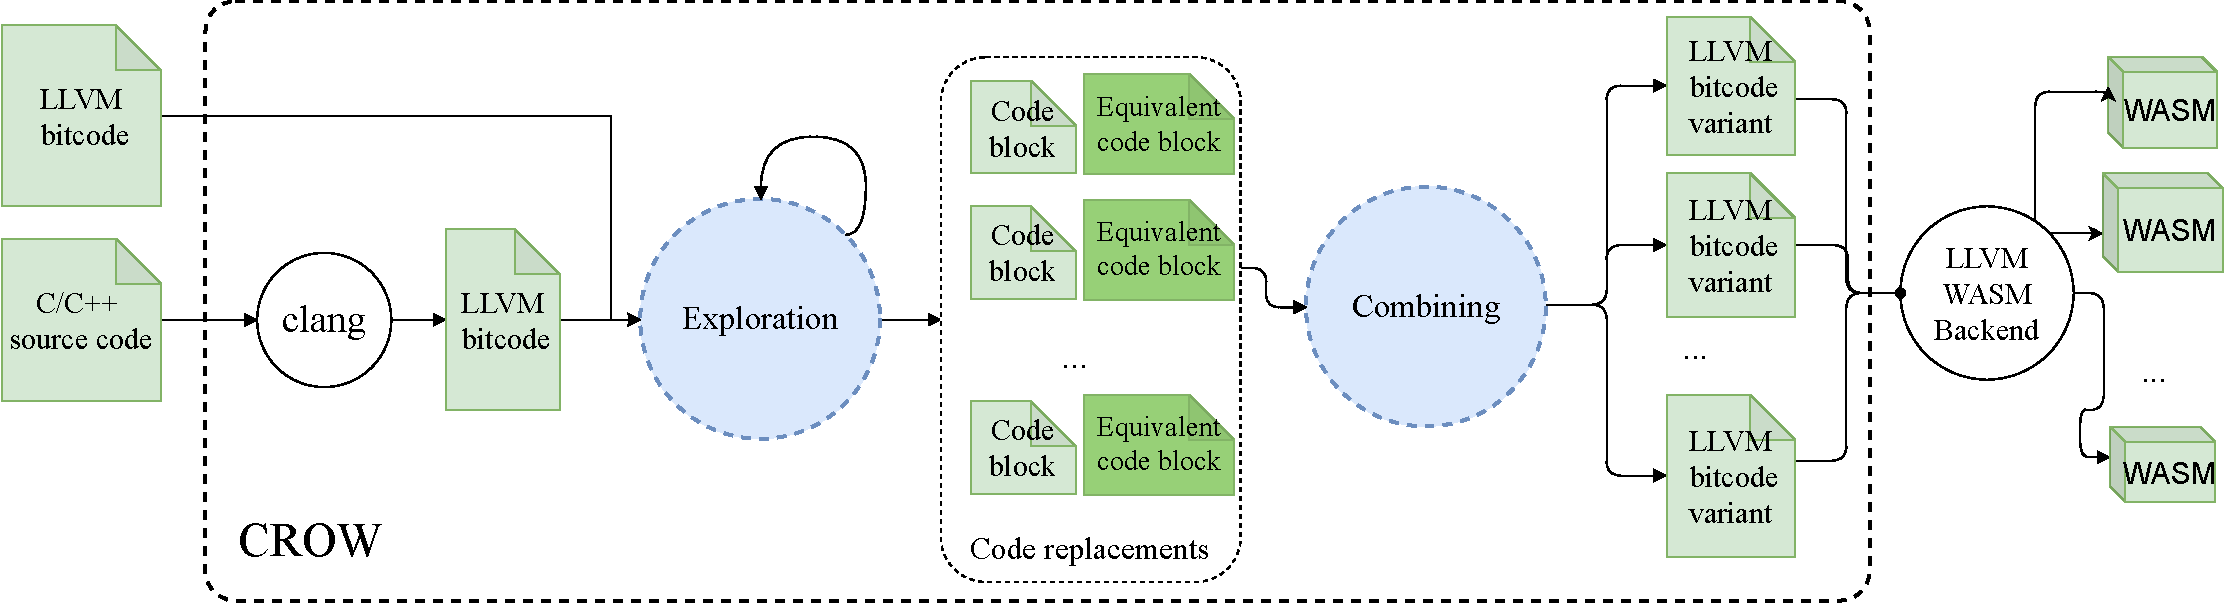
\includegraphics[width=\linewidth]{diagrams/generation/crow.drawio.pdf}
    \caption{CROW workflow to generate program variants. CROW takes C/C++ source codes or LLVM bitcodes to look for code blocks that can be replaced by semantically equivalent code and generates program variants by combining them.}
    \label{diagrams:crow}
\end{figure*}



%CROW operates at the code block level, taking them from the functions defined inside the input LLVM bitcode module. 
%In addition, the retargeted superoptimizer is in charge of finding the potential places in the original code blocks where a replacement can be applied. Finally, we use the enumerative synthesis strategy of the retargeted superoptimizer to generate code replacements.
%The code replacements generated through synthesis are verified, according to \autoref{def:functional-equivalence}, by internally using a theorem prover. 

\begin{comment}

\begin{definition}{Block (based on Aho \etal \cite{ahodragonbook}):}\label{def:code-block}
    Let $P$ be a program. A block $B$ is a grouping of declarations and statements in $P$ inside a function $F$. 
\end{definition}

\todo{Move to chapter 2}

\begin{definition}{Functional equivalence modulo program state (based on Cohen \etal \cite{cohen1993operating}):}
    \label{def:functional-equivalence}
    Let $B_1$ and $B_2$ be two code blocks according to \autoref{def:code-block}. We consider the program state before the execution of the block, $S_i$, as the input and the program state after the execution of the block, $S_o$, as the output. $B_1$ and $B_2$ are functionally equivalent if given the same input $S_i$ both codes produce the same output $S_o$.
\end{definition}

\begin{definition}{Code replacement:}
    \label{def:code-replacement}
    Let $P$ be a program and $T$ a pair of code blocks $(B_1, B_2)$. $T$ is a candidate code replacement if $B_1$ and $B_2$ are both functionally equivalent as defined in \autoref{def:functional-equivalence}.
    Applying $T$ to $P$ means replacing $B_1$ by $B_2$. The application of $T$ to $P$ produces a program variant $P'$ which consequently is functionally equivalent to $P$.     
\end{definition}
\end{comment}

\subsection*{Variants' generation}

CROW is based on the work of Jacob \etal \cite{jacob2008superdiversifier}. Their work uses code superoptimization to generate software diversification with an approach called superdiversification. 
% How a superoptimizer works
Code superoptimization focuses on \emph{searching} for a new program which is faster or smaller than the original code, while preserving its functionality.
The concept of superoptimizing a program dates back to 1987, with the seminal work of Massalin \cite{Massalin1987} which proposes an exhaustive exploration of the solution space. The search space is defined by choosing a subset of the machine's instruction set and generating combinations of optimized programs, sorted by length in ascending order. If any of these programs are found to perform the same function as the source program, the search halts. The main difference between the superoptimization process and a superdiversifier it that the latter keeps intermediate search results for the sake of diversification. 

We use the seminal work of Jacob and colleagues to implement CROW because of two main reasons.
First, the code replacements generated by this technique outperform diversification strategies based on hand-written rules. Besides, this technique is fully automatic.
Second, there is a battle tested superoptimizer for LLVM, Souper \cite{Sasnauskas2017Souper:Superoptimizer}. It dates from 2017 and has an active community of maintainers. By extending Souper with superdiversification, it allows us to contribute with a new mutation strategy, \emph{constant inferring} (in addition to the before mentioned strategies in \autoref{sota:sota}) to artificially generate diversification. We modify it to keep the intermediate solutions in their searching algorithm to generate program variants. Besides, 
we prevent Souper from synthesizing instructions that have no correspondence in the \wasm backend to reduce the searching space for variants. In addition, we disable the majority of the pruning strategies of Souper for the sake of more variants. Our modified version of Souper can be found at \todo{}.

% Souper
%Souper is an state-of-the-art superoptimizer for LLVM. It enumerates a set of several optimization candidates to be replaced.
%Souper is based on a Satisfiability Modulo Theories (SMT) solver. SMT solvers are useful for both verification and synthesis of programs \cite{10.1007/978-3-540-78800-3_24}.

%We implement the \emph{exploration} stage of CROW by retargeting Souper. The main objective of Souper is to find the best (smallest) possible program,  

\subsection*{Constant inferring}

As we previously mentioned, extending Souper as a superdiversifier contributes with a new mutation strategy called \emph{constant inferring}. 
The main component of Souper infers pieces of code as a single constant assignment particularly for boolean valued variables that are used to control branches.
If a program branching is removed due to a constant inferring, the generated program is considerably different to the original program, statically and dynamically.
Let us illustrate the case with an example.
The Babbage problem code is composed of a loop which stops when it discovers the smaller number that fits with the Babbage condition below.
\begin{center}
\begin{tabular}{c}

\lstset{language=C++,
                    style=CStyle,
                    basicstyle=\small\ttfamily,
                    columns=fullflexible,
                    breaklines=true, 
                    postbreak=\mbox{\textcolor{red}{$\hookrightarrow$}\space}}
\begin{lstlisting}[]
while((n * n) % 1000000 != 269696) n++;
\end{lstlisting}
\end{tabular}
\end{center}
% llvm-opt: rool unroll
In theory, this value can also be inferred by unrolling the loop the correct number of times with traditional tools like llvm-opt.
However, llvm-opt cannot unroll a \texttt{\textbf{while}}-loop because the loop count is too large.
% Souper
On the other hand, Souper can deal with this case, inferring the value of $n$ such that the Babbage condition is reached. Therefore, since the condition in the loop will always be false, the loop is dead code, and is removed in the final compilation. It is clear that the new program is remarkably different, smaller and faster than the original code.

When we retarget Souper we recombine all found replacements to create new programs, including those for which a constant inferring was performed.
This allows to create variants that are also better than the original program in terms of size and performance.

\subsection*{Removing latter optimizations for LLVM}

During the implementation of CROW we have the premise of removing all builtin optimizations in the LLVM compiler that could reverse Wasm variants.
Therefore, in addition to the extension of Souper, we modify the LLVM compiler and the \wasm backend.
We disable all optimizations in the \wasm backend that could reverse the superoptimizer transformations, such as constant folding and instructions normalization.


%\todo{We disable cost restrictions and the LLVM backend optimizations...maybe for the assesment RQ ?}

\subsection*{CROW instantiation}
%\label{section:crow:example}
%In \autoref{section:crow} we describe the main components and contributions of CROW. In this section we instantiate the workflow presented in \autoref{workflow} from the input of an example C code to the generation of a pool of \wasm program variants.

Let us illustrate how CROW works with the simple example code in \autoref{CExample}. The \texttt{f} function calculates the value of $2 * x + x$ where \texttt{x} is the input for the function.  CROW compiles this source code and generates the intermediate LLVM bitcode in the left most part of \autoref{example:crow:original:llvm}. CROW potentially finds two code blocks to look for variants, as the right-most part of \autoref{example:crow:original:llvm} shows.

% snippet of code showing the detection of code blocks
    
\begin{code}
    \lstset{language=C,
    basicstyle=\small\ttfamily,caption={C function that calculates the quantity $2x + x$},label=CExample}
    \begin{lstlisting}[style=CStyle]
int f(int x) { 
    return 2 * x + x; 
}    
    \end{lstlisting}
    
\end{code}

\lstdefinelanguage{LLVM}
    {morekeywords={i32,mul,align,nsw,add,load,store,define,br, ret, shl, ret},
    sensitive=false,
    morecomment=[l]{;},
    morecomment=[s]{;}{;},
    morestring=[b],
}
\lstdefinestyle{nccode}{
    numbers=left,
    tabsize=4,
    showspaces=false,
    breaklines=true, 
    showstringspaces=false,
    moredelim=**[is][{\btHL[fill=black!10]}]{`}{`},
    moredelim=**[is][{\btHL[fill=celadon!40]}]{!}{!}
}
\lstset{
    language=LLVM,
    style=nccode,
    %basicstyle=\small\ttfamily,
    columns=fullflexible,
    breaklines=true
}


\begin{code}
    \centering
    \captionof{lstlisting}{LLVM's intermediate representation program, its extracted instructions and replacement candidates. Gray highlighted lines represent original code, green for code replacements. }\label{example:crow:original:llvm}
    \lstset{numbers=none}
    \noindent\begin{minipage}[t]{.33\linewidth}
    \centering
    \begin{lstlisting}[xleftmargin=1em,escapechar=?]
    define i32 @f(i32) {

    ?\tikzmarkWS{2}{code 2}{11.5}{10}{3.5cm}?
    ?\tikzmarkWS{1}{code 1}{11.5}{3.5}{3.0cm}?
    %2 = mul nsw i32 %0,2
    %3 = add nsw i32 %0,%2 

    ret i32 %3
    }
    
    define i32 @main() {
    %1 = tail call i32 @f(i32 10)
    ret i32 %1
    }
    \end{lstlisting}
    \end{minipage}%\hfill%
    \begin{minipage}[t]{.32\linewidth}
        \begin{lstlisting}[xleftmargin=1em,escapechar=?]
?Replacement candidates for code\_1?

`%2 = mul nsw i32 %0,2`

!%2 = add nsw i32 %0,%0!

!%2 = shl nsw i32 %0, 1:i32!
    \end{lstlisting}
    \end{minipage}%\hfill%
    \begin{minipage}[t]{.32\linewidth}
        \lstdefinestyle{nccode}{
        tabsize=4, 
        showspaces=false,
        breaklines=true, 
        showstringspaces=false,
        moredelim=**[is][{\btHL[fill=black!10]}]{`}{`},
        moredelim=**[is][{\btHL[fill=celadon!40]}]{!}{!}
        }
        \lstset{
            language=LLVM,
            style=nccode,
            columns=fullflexible,
            breaklines=true,
            belowcaptionskip=1pt,
            abovecaptionskip=1pt,
        } 
        \begin{lstlisting}[name={B},escapechar=?]
?Replacement candidates for code\_2?

`%3 = add nsw i32 %0,%2`

!%3 = mul nsw %0, 3:i32!
        \end{lstlisting}
    \end{minipage}
    
\end{code}





\begin{code}
    \centering
    \captionof{lstlisting}{Candidate code replacements combination. Orange highlighted code illustrate replacement candidate overlapping.}\label{example:crow:original:combination}
    \lstset{numbers=none}
    \noindent\begin{minipage}[t]{.5\linewidth}
    \begin{lstlisting}[xleftmargin=1em,escapechar=?]
`%2 = mul nsw i32 %0,2`
`%3 = add nsw i32 %0,%2`

!%2 = add nsw i32 %0,%0!
`%3 = add nsw i32 %0,%2`

!%2 = shl nsw i32 %0, 1:i32!
`%3 = add nsw i32 %0,%2`

    \end{lstlisting}
    \end{minipage}%\hfill%
    \begin{minipage}[t]{.5\linewidth}
        \lstdefinestyle{nccode}{
        tabsize=4, 
        showspaces=false,
        breaklines=true, 
        showstringspaces=false,
        moredelim=**[is][{\btHL[fill=black!10]}]{`}{`},
        moredelim=**[is][{\btHL[fill=celadon!40]}]{!}{!},
        moredelim=**[is][{\btHL[fill=weborange!40]}]{'}{'}
        }
        \lstset{
            language=LLVM,
            style=nccode,
            columns=fullflexible,
            breaklines=true,
            belowcaptionskip=1pt,
            abovecaptionskip=1pt,
        } 
        \begin{lstlisting}[xleftmargin=1em,escapechar=?]
'%2 = mul nsw i32 %0,2'
!%3 = mul nsw %0, 3:i32!

'%2 = add nsw i32 %0,%0'
!%3 = mul nsw %0, 3:i32!

'%2 = shl nsw i32 %0, 1:i32'
!%3 = mul nsw %0, 3:i32!

    \end{lstlisting}
    \end{minipage}
\end{code}


\begin{tikzpicture}[remember picture,overlay]
%\path (2.north) edge[<-, bend left] (1.north);
%\path[draw, ->] (3.west) edge[<-, bend left] (2.west);
%\path (4.west) edge[<-, bend left] (3.west);
%\path (1.south) edge[<-, bend left] (4.south);

%\path (2.east) edge[<-, bend left, blue] (5.north);
%\path (3.east) edge[<-, bend right, olive] (2.east);
%\path (1.east) edge[<-, bend left, black] (replall1.west);
%\path (2.east) edge[<-, bend left, black] (replall2.west);
%\path (rep11.east) edge[<-, bend left, black] (6.east);
%\path (9.east) edge[<-, bend right, black] (4.east);
%\path (7.east) edge[<-, bend right, black] (8.east);
%\path (5.south) edge[<-, bend right, blue] (4.east);
%\path (9.north) edge[<-] (8.south);
%\path (5.south) edge[<-, bend left] (9.south);


%\path (10.north) edge[<-, bend left] (11.north);
%\path (11.south) edge[<-, bend left] (10.south);
%\path (7) edge[<-, bend right] (6.east);
%\path (8) edge[<-, bend right] (7.east);
\end{tikzpicture}


    

CROW, in the exploration stage detects 2 code blocks, \texttt{code\_block\_1} and \texttt{code\_block\_2} as the enclosing boxes in the left most part of \autoref{example:crow:original:llvm} shows. CROW synthesizes $2 + 1$ candidate code replacements for each code block respectively as the green highlighted lines show in the right most parts of \autoref{example:crow:original:llvm}.
The baseline strategy of CROW is to generate variants out of all possible combinations of the candidate code replacements, \ie uses the power set of all candidate code replacements.

In the example, the power set is the cartesian product of the found candidate code replacements for each code block, including the original ones, as \autoref{example:crow:original:combination} shows. The power set size results in $6$ potential function variants. Yet, the generation stage would eventually generate $4$ variants from the original program. CROW generated 4 statically different Wasm files, as \autoref{example:crow:variants:wasm} illustrates. This gap between the potential and the actual number of variants is a consequence of the redundancy among the bitcode variants when composed into one. In other words, if the replaced code removes other code blocks, all possible combinations having it will be in the end the same program. In the example case, replacing \texttt{code\_block\_2} by \texttt{mul nsw \%0, 3}, turns \texttt{code\_block\_1} into dead code, thus, later replacements generate the same program variants. The rightmost part of \autoref{example:crow:original:combination} illustrates how for three different combinations, CROW produces the same variant. We call this phenomenon a candidate code replacement overlapping.

One might think that a reasonable heuristic could be implemented to avoid such overlapping cases. Instead, we have found it easier and faster to generate the variants with the combination of the replacement and check their uniqueness after the program variant is compiled. This prevents us from having an expensive checking for overlapping inside the CROW code. Still, this phenomenon calls for later optimizations in future works.

\lstdefinestyle{nccode}{
        numbers=none,
        firstnumber=2,
        stepnumber=1,
        numbersep=10pt,
        tabsize=4, 
        showspaces=false,
        breaklines=true, 
        showstringspaces=false,
    moredelim=**[is][\btHL]{`}{`},
    moredelim=**[is][{\btHL[fill=black!10]}]{`}{`},
    moredelim=**[is][{\btHL[fill=celadon!40]}]{!}{!}
}

\lstset{
    language=WAT,
    style=nccode,
    basicstyle=\footnotesize\ttfamily,
    columns=fullflexible,
    breaklines=true
}


\begin{code}
    \centering
    \captionof{lstlisting}{\termidx{Wasm }program variants generated from program \autoref{CExample}.}\label{example:crow:variants:wasm}
    \lstset{numbers=none}
    \noindent\begin{minipage}[t]{.45\linewidth}
    \begin{lstlisting}[xleftmargin=1em,escapechar=?]
func $f (param i32) (result i32)
   local.get 0
    `i32.const 2`
    `i32.mul`
    `local.get 0`
    `i32.add`

        \end{lstlisting}
\begin{lstlisting}[xleftmargin=1em,escapechar=?]
func $f (param i32) (result i32)
    local.get 0
    !local.get 0!
    !i32.add!
    `local.get 0`
    `i32.add`

                \end{lstlisting}
    \end{minipage}\hfill
    \noindent\begin{minipage}[t]{.45\linewidth}
\begin{lstlisting}[xleftmargin=1em,escapechar=?]
func $f (param i32) (result i32)
    local.get 0
    !i32.const 1!
    !i32.shl!
    `local.get 0`
    `i32.add`

    \end{lstlisting}
\begin{lstlisting}[xleftmargin=1em,escapechar=?]
func $f (param i32) (result i32)
    local.get 0
    !i32.const 3!
    !i32.mul!

            \end{lstlisting}
        \end{minipage}
\end{code}





\section{MEWE: Multi-variant Execution for WEbAssembly}
\label{section:mewe}

\newcommand{\tool}{MEWE\xspace}
\newcommand{\repourl}{TODO}
% Overview
This section describes MEWE \cite{MEWE}, our second contribution. 
%MEWE is implemented in 942 lines of C++ code.
The core idea of \tool is to synthesize diversified function variants, using CROW, providing execution-path randomization in an MVE.
The tool generates application-level multivariant binaries, without any change to the operating system or \wasm runtime.
%It uses the LLVM 12.0.0 libraries to extend the LLVM standard linker tool capability with the multivariant generation.
%Per Crane et al. the execution-path randomization is made to hinder side-channel attacks \cite{crane2015thwarting}. 
% All programs are diversified with behavior preservation guarantees according to the design of CROW (\autoref{section:crow}).
MEWE creates an MVE by intermixing functions for which CROW generates variants, as step \step{2} in \autoref{diagrams:generic} shows.
CROW generates each one of these variants with fine-grained diversification at instruction level, applying the majority of the strategies discussed in \autoref{sota:sota} and \emph{constant inferring}. Besides, \tool inlines function variants when appropriate, also resulting in call stack diversification at runtime.

In \autoref{workflow} we zoom MEWE(\step{4}) from the diagram in \autoref{diagrams:generic}. MEWE takes the LLVM IR variants generated by our diversifier and merges them into a Wasm multivariant.
In the figure, we highlight the two components of MEWE. 
In Step~\step{I}, we merge the LLVM IR variants created by CROW and we create a LLVM multivariant binary.
In Step~\step{II}, we use a special component, called a ``Mixer``,  which augments the binary with a random generator, which is required for performing the execution-path randomization. 
Also at this stage, the multivariant binary is fixed with the entrypoint of the original binary.
%The harness is used to connect the program to its original execution environment while the generator provides support for random execution path at runtime.
The final output of Step~\step{III} is a standalone multivariant \wasm binary that can be directly deployed. 
%For sake of open science and for fostering research on this important topic, the code of \tool is made publicly available on GitHub: \repourl.

\begin{figure*}
  \centering
  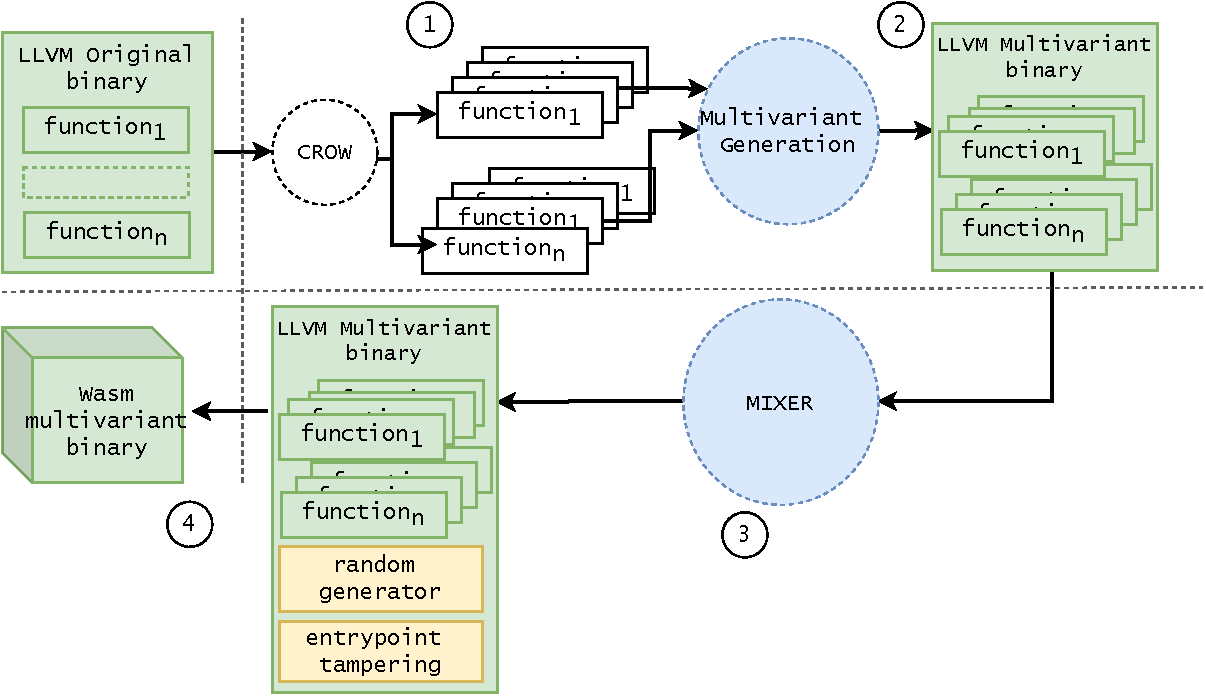
\includegraphics[height=3.1in]{diagrams/MEWE.pdf}
  \caption{Overview of \tool. It takes as input an LLVM binary. It first generates a set of functionally equivalent variants for each function in the binary and then generates a LLVM multivariant binary composed of all the function variants. Also, it includes the dispatcher functions in charge of selecting a variant when a function is invoked. The \tool mixer composes the LLVM multivariant binary with a random number generation library and a tampering of the original application entrypoint, in order to produce a \wasm multivariant binary ready to be deployed. }
  \label{workflow}
\end{figure*}


\subsection*{Multivariant generation}

The key component of \tool consists in combining the variants into a single binary.
The goal is to support execution-path randomization at runtime.
% General idea
The core idea is to introduce one dispatcher function per original function with variants.
A dispatcher function is a synthetic function that is in charge of choosing a variant at random, every time the original function is invoked during the execution.
With the introduction of dispatcher function,  \tool turns the original call graph into a multivariant call graph, defined as follows. 

\begin{definition}{Multivariant Call Graph (MCG):}\label{def:EP}
  
    A multivariant call graph is a call graph $\langle N,E \rangle$ where the nodes in $N$ represent all the functions in the binary and an edge $(f_1,f_2) \in E$ represents a possible invocation of $f_2$ by $f_1$  \cite{ryder1979}, where the nodes are typed. The nodes in $N$ have three possible types: a function present in the original program,  a generated function variant, or a dispatcher function.
\end{definition}


\begin{figure}
    \centering
  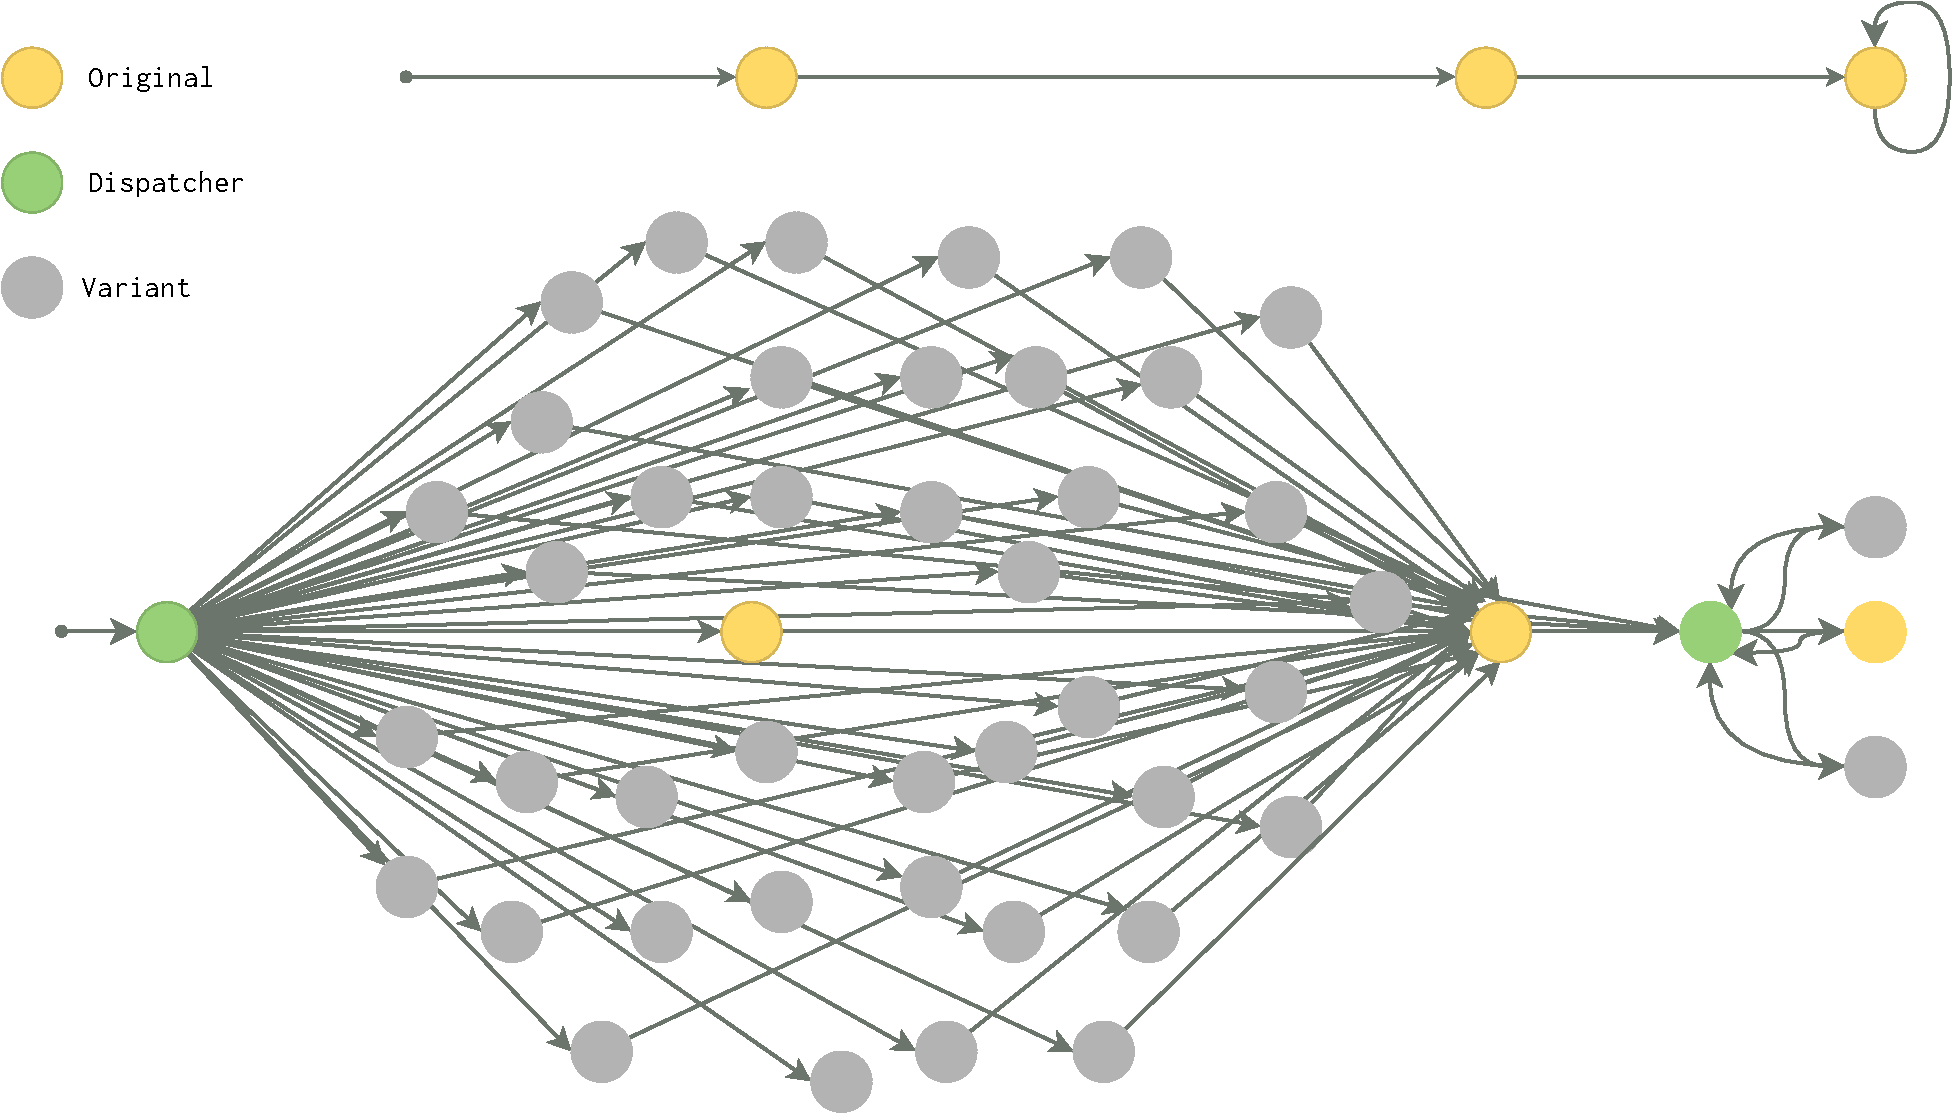
\includegraphics[width=.8\linewidth]{diagrams/CFG.pdf}
  \caption{Example of two static call graphs. At the top, the original call graph, at the bottom, the multivariant call graph, which includes nodes that represent function variants (in grey), dispatchers (in green), and original functions  (in yellow).
}
  \label{multivariant}
\end{figure}

% Instance of a multivariant module
In \autoref{multivariant}, we show the original static call graph for and original program (top of the figure), as well as the multivariant call graph generated with \tool (bottom of the figure).
The grey nodes represent function variants, the green nodes function dispatchers and the yellow nodes are the original functions.
The possible calls are represented by the directed edges.
The original program includes 3 functions. \tool generates 43 variants for the first function, none for the second and three for the third function. 
\tool introduces two dispatcher nodes, for the first and third functions. Each dispatcher is connected to the corresponding function variants, in order to invoke one variant randomly at runtime.


% exaplanation of dispatcher
In  \autoref{listing:multivariant_template}, we illustrate the LLVM construction for the function dispatcher corresponding to the right most green node of \autoref{multivariant}.
% General logic of a multivartiant function
It first calls the random generator, which returns a value that is then used to invoke a specific function variant. 
% Why a linear based switch
We implement the dispatchers with a switch-case structure to avoid indirect calls that can be susceptible to speculative execution based attacks \cite{Narayan2021Swivel}. 
The choice of a switch-case also avoids having multiple function definitions with the same signature, which could increase the attack surface in case the function signature is vulnerable \cite{johnson2021}.
This also allows \tool to inline function variants inside the dispatcher, instead of defining them again.
Here we trade security over performance, since dispatcher functions  that perform indirect calls, instead of a switch-case,  could improve the performance  of the dispatchers as indirect calls have constant time.
%It should be noted that the dispatcher function is constructed using the same signature as the original function. 


\lstset{
    language=llvm,
    %style=nccode,
    basicstyle=\footnotesize\ttfamily,
    columns=fullflexible,
    breaklines=true,
    numbers=none,
    stepnumber=1,
    float
}

\begin{code}
\scriptsize
\noindent\begin{minipage}[b]{\linewidth}
    \begin{minipage}[t]{1\linewidth}
        \begin{lstlisting}[escapeinside={(*}{*)}]
define internal i32 @foo(i32 %0) {
    entry:
      %1 = call i32 @discriminate(i32 3)
      switch i32 %1, label %end [
        i32 0, label %case_43_
        i32 1, label %case_44_
      ]
    case_43_:                 
      %2 = call i32 @foo_43_(%0)
      ret i32 %2
    case_44_:                
      %3 = <body of foo_44_ inlined>
      ret i32 %3
    end:                                             
      %4 = call i32 @foo_original(%0)
      ret i32 %4
}
        \end{lstlisting}
    \end{minipage}%
    
    \noindent\rule{\linewidth}{0.4pt}
    \captionof{lstlisting}{Dispatcher function embedded in the multivariant binary of the original function in the rightmost green node in \autoref{multivariant}.}\label{listing:multivariant_template}
\end{minipage}
\end{code}

\subsection*{Mixer}

The Mixer has four specific objectives: tamper the entrypoint of the application, link the LLVM multivariant binary, inject a random generator and merge all these components into a multivariant \wasm binary.
% Implementation
We use the Rustc compiler\footnote{\url{https://doc.rust-lang.org/rustc/what-is-rustc.html}} to orchestrate the mixing.
% The random number generation
For the random generator, we rely on WASI's specification \cite{WASI} for the random behavior of the dispatchers. Its exact implementation is dependent on the platform on which the binary is deployed.

The \tool mixer creates a new entrypoint for the binary called \emph{entrypoint tampering}.
It simply wraps the dispatcher for the entrypoint variants as a new function for the final Wasm  binary and is declared as the application entrypoint. %This fixes an issue with  

% How to turn function into endpoints
%The entrypoint tampering is needed for binariess passed to MEWE. We refer to the entrypoint as the entering main function of the original binary passed to MEWE. The tampering is needed because dispatchers for entrypoint variants make the multivariant invalid to be directly executed after it is compiled to Wasm.

%Throughout this paper, we refer to an endpoint as the closure of invoked functions when the entry point of the \wasm binary is executed.



\begin{comment}

\subsection{Multivariant Binary Execution at the Edge}

\todo{Introduce as the use of MEWE}

% What really is executed is the x86 code
When a WebAssembly binary is deployed on an edge platform, it is translated to machine code on the fly.
For our experiment, we deploy on the production edge nodes of Fastly. This edge computing platform uses Lucet, a native WebAssembly compiler and runtime, to compile and run the deployed Wasm  binary \footnote{\url{https://github.com/bytecodealliance/lucet}}.
Lucet generates x86 machine code and ensures that the generated machine code executes inside a secure sandbox, controlling memory isolation.


\begin{figure}
\centering
  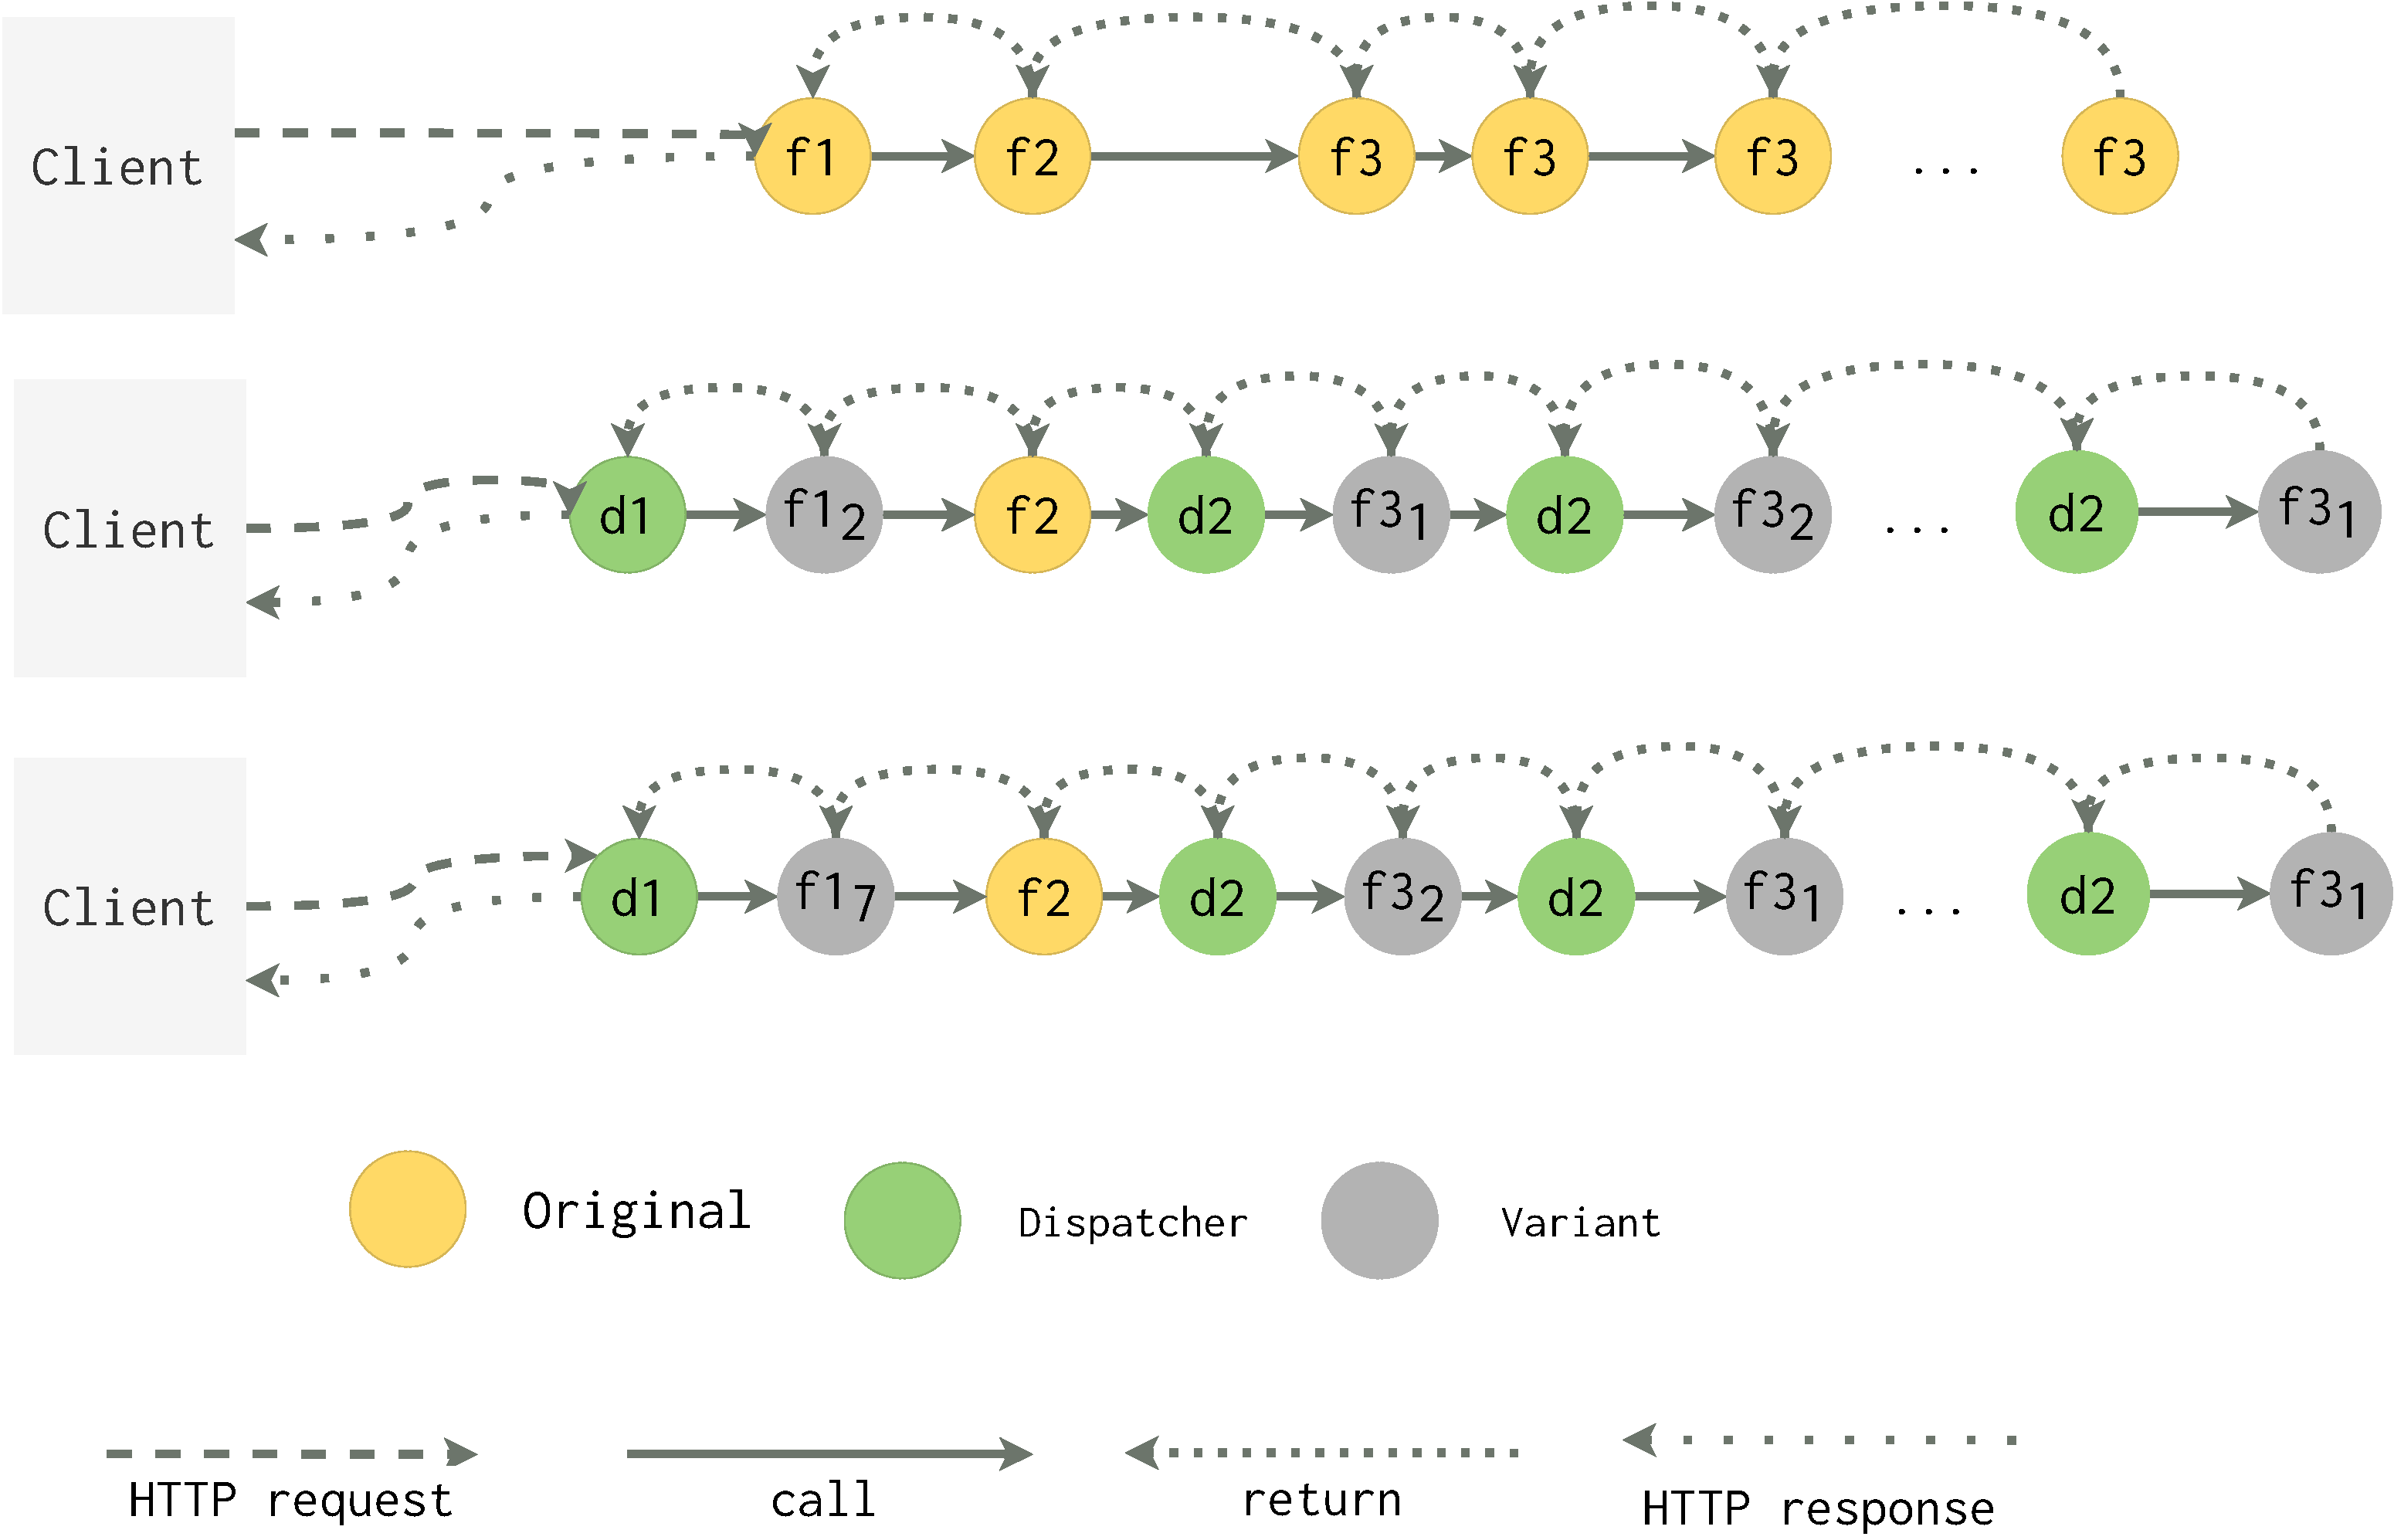
\includegraphics[width=1\linewidth]{diagrams/traces.pdf}
  \caption{Top: an execution trace for the  \texttt{bin2base64} endpoint. Middle and bottom: two different execution traces for the multivariant \texttt{bin2base64}, exhibited by two different requests with exactly the same input.}
  \label{http:workflow}
\end{figure}

% How it works
\autoref{http:workflow} illustrates  the runtime behavior of the original and the multivariant binary,  when deployed on an Edge node.
The top most diagram illustrates the execution trace for the  original of the endpoint \texttt{bin2base64}.
When the HTTP request with the input \texttt{"Hello World!"} is received, it invokes functions $f1$, $f2$ followed by 27 recursive calls of function $f3$. Then, the endpoint sends the result \texttt{"0x000xccv0x10x00b3Jsx130x000x00 0x00xpopAHRvdGE="} of its base64 encoding in an HTTP response.

The two diagrams at the bottom of \autoref{http:workflow} illustrate two executions traces observed through two different requests to the endpoint \texttt{bin2base64}.
In the first case, the request first triggers the invocation of dispatcher $d1$, which randomly decides to invoke the variant $f1_2$; then $f2$, which has not been diversified by \tool, is invoked; then the recursive invocations to $f3$ are replaced by iterations over the execution of dispatcher $d2$ followed by a random choice of variants of $f3$. Eventually the result is computed and sent back as an HTTP response. 
The second execution trace of the multivariant binary shows the same sequence of dispatcher and function calls as the previous trace, and also shows that for a different requests, the variants of $f1$ and $f3$ are different. 


The key insights from these figures are as follows. First, from a client's point of view, a request to the original or to a multivariant endpoint, is completely transparent. Clients send the same data, receive the same result, through the same protocol, in both cases.
Second, this figure shows that, at runtime, the execution paths for the same endpoint are different from one execution to another, and that this randomization process results from multiple random choices among function variants, made through the execution of the endpoint.
%From an attacker's perspective, this random selection of variants constantly moves the attack surface and is meant to render a potential vulnerability harder to reach or exploit \cite{davi2015isomeron, 10.5555/3091125.3091155, BEKIROGLU2021106601}.


\end{comment}




\section*{Conclusions}

This chapter discusses the technical details for the artifacts implemented for our two contributions.
We describe how \termidx{CROW }generates program variants.
We introduce a new mutation strategy that is a consequence of retargeting a superoptimizer for LLVM as a superdiversifier.
Besides, we dissect \termidx{MEWE }and how it creates an MVE system.
In \autoref{chapter:method} we discuss the methodology we follow to evaluate the impact of \termidx{CROW }and MEWE.